% German USTVA template for taxreports
% Contributed by Jacky und Stefan Tenne 
% Based on template by Jens Koerner, Peter Schorer, Udo Spallek
%
%
\documentclass[twoside]{scrartcl}
\usepackage{a4,german}
\usepackage[frame]{xy}
\usepackage[utf8]{inputenc}
\usepackage[german]{babel}
\usepackage{graphicx}
\usepackage{tabularx}
\usepackage{times, german}
\usepackage{german}
\setlength{\voffset}{-0.7cm} %hier wird die Höhenverschiebung getÀtigt
\setlength{\hoffset}{-1cm}  %und hier die Verschiebung seitwÀrts
\setlength{\topmargin}{0cm}
\setlength{\headheight}{0cm}
\setlength{\headsep}{0cm}
\setlength{\topskip}{0pt}
\setlength{\oddsidemargin}{0cm}
\setlength{\evensidemargin}{0cm}
\setlength{\textwidth}{20.9cm}
\setlength{\textheight}{29.6cm}
\setlength{\footskip}{-0cm}
\setlength{\parindent}{1mm}

\begin{document}

\fontfamily{cmss}\fontshape{n}\large\selectfont
\pagestyle{myheadings}
\markboth{\protect\scalebox{1.045}[1.045]{\protect\includegraphics[viewport = 54 783 700 790,page=2]{ustva-2008.pdf}}}%Seite 2
{\protect\scalebox{1.045}[1.045]{\protect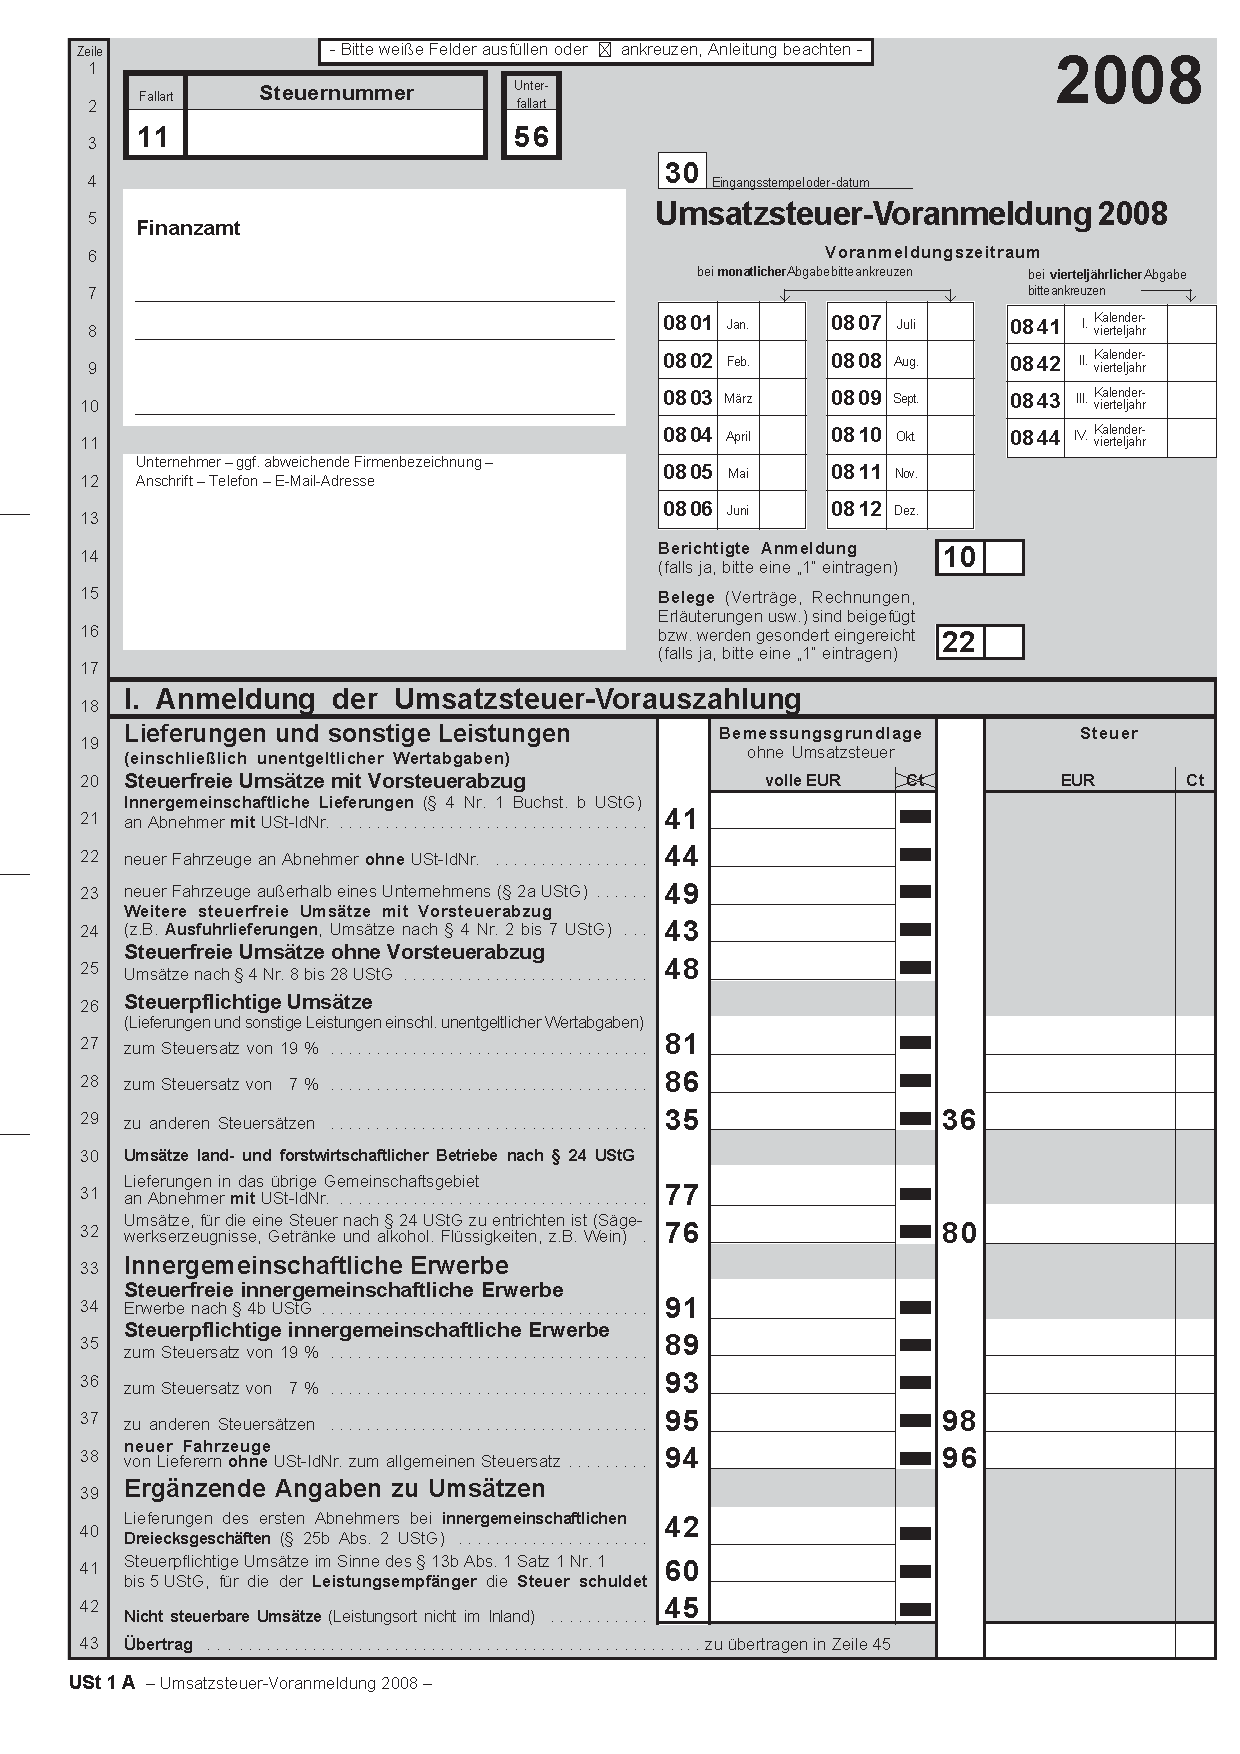
\includegraphics[viewport = 70 700 700 790,page=1]{ustva-2008.pdf}}}%Seite 1
\hspace{1mm}
\begin{tabular}[b]{p{7mm}p{5cm}p{22.5mm}p{24mm}p{7mm}p{28mm}p{3mm}}
\multicolumn{7}{c}{}\\[-2mm]
 &  \multicolumn{6}{l}{<%steuernummer%>}\\
\multicolumn{7}{c}{}\\[15mm]
\multicolumn{2}{p{7.5cm}}{<%FA_Name%>} & & & & &\\[-4mm]
\multicolumn{2}{p{7.5cm}}{}  & & & & &\\[3mm]
\multicolumn{2}{p{7.5cm}}{<%FA_Strasse%>} & &<%0401%>&<%0407%>&&<%0441%>\\[1.2mm]
\multicolumn{2}{p{7.5cm}}{} & &<%0402%>&<%0408%>&&<%0442%>\\[1.25mm]
\multicolumn{2}{p{7.5cm}}{<%FA_PLZ%> <%FA_Ort%>} & &<%0403%>&<%0409%>&&<%0443%>\\[3mm]
\multicolumn{2}{p{7.5cm}}{} & &<%0404%>&<%0410%>&&<%0444%>\\[1.25mm]
\multicolumn{2}{p{7.5cm}}{} & &<%0405%>&<%0411%>&&\\[1.25mm]
\multicolumn{2}{p{7.5cm}}{\small{<%company%>}} & &<%0406%>&<%0412%>&&\\[-1mm]
\multicolumn{2}{p{7.5cm}}{\small{<%co_street%>}}& & & & &\\[-1mm]
\multicolumn{2}{p{7.5cm}}{\small{<%co_city%>}}& & & &<%FA_10%> &\\[1mm]
\multicolumn{2}{p{7.5cm}}{
<%if tel%>
\small{Tel: <%tel%>}~--~
<%end tel%>
<%if fax%>
\small{Fax: <%fax%>}
<%end fax%>
}& & & & &\\[1.8mm]
\multicolumn{2}{p{7.5cm}}{\small{<%email%>}}& & & & &\\[-1mm]
\end{tabular}\\[29.5mm]
\begin{tabular}[b]{p{99mm}p{26.5mm}p{4.55mm}p{4mm}p{35mm}}
&&&&\\[15.6mm]
\multicolumn{2}{r}{<%48%>} & & \multicolumn{2}{r}{}\\[8.5mm]
\multicolumn{2}{r}{<%81%>} & & \multicolumn{2}{r}{<%811%>}\\[1.8mm]
\multicolumn{2}{r}{<%86%>} & & \multicolumn{2}{r}{<%861%>}\\[41.7mm]
\multicolumn{2}{r}{<%97%>} & & \multicolumn{2}{r}{<%971%>}\\[1.5mm]
\multicolumn{2}{r}{<%93%>} & & \multicolumn{2}{r}{<%931%>}\\[8.5mm]
\multicolumn{2}{r}{<%94%>} & & \multicolumn{2}{r}{<%96%>}\\[28.5mm]
\multicolumn{2}{r}{} & & \multicolumn{2}{r}{<%Z43%>}\\
\end{tabular}
\newpage

\vspace*{-9.5mm}\hspace{27mm}<%steuernummer%>\\[-2.7mm]
\begin{tabular}[b]{p{99mm}p{25.2mm}p{2.55mm}p{10mm}p{32mm}}
&&&&\\[0.75mm]
\multicolumn{2}{r}{} & & \multicolumn{2}{r}{<%Z45%>}\\[48.3mm]
\multicolumn{2}{r}{} & & \multicolumn{2}{r}{<%Z53%>}\\[8.4mm]
\multicolumn{2}{r}{} & & \multicolumn{2}{r}{<%66%>}\\[41.7mm]
\multicolumn{2}{r}{} & & \multicolumn{2}{r}{<%Z62%>}\\[28.4mm]
\multicolumn{2}{r}{} & & \multicolumn{2}{r}{\textbf{<%83%>}}\\[25.6mm]
\end{tabular}\\[35mm]
<%if FA_steuerberater%>
\vspace{11mm}
\begin{list}{}{
\setlength{\leftmargin}{2mm}
\setlength{\itemsep}{0mm}
\setlength{\parsep}{0mm}
%\setlength{\topsep}{0mm}
%\setlength{\parskip}{0mm}
%\setlength{\partopsep}{0mm}
}
\begin{small}
\item <%FA_steuerberater_name%>
\item <%FA_steuerberater_street%>
\item <%FA_steuerberater_city%>
\item Tel:~<%FA_steuerberater_tel%>
\end{small}\\[15mm]
\item  <%Datum_heute%>,
\end{list}
<%end FA_steuerberater%>
<%if not FA_steuerberater%>
\begin{list}{}{
\setlength{\leftmargin}{2mm}
\setlength{\itemsep}{0mm}
\setlength{\parsep}{0mm}
%\setlength{\topsep}{0mm}
%\setlength{\parskip}{0mm}
%\setlength{\partopsep}{0mm}
}
\begin{small}
\item ~
\item ~
\item ~
\item ~
\end{small}\\[26mm]
\item  <%Datum_heute%>,
\end{list}
<%end FA_steuerberater%>
\end{document}










